\documentclass{beamer}
\usepackage{EnglishSlides}

\begin{document}

\title[Reliable Scalable Maintainable Apps]{Reliable Scalable Maintainable Applications}
\author[Hrachya Tandilyan\copyright]{Hrachya Tandilyan}
\date{2020}

%-------------------------------------------------------------------------------------------------
\begin{frame}
\titlepage
\end{frame}
%-------------------------------------------------------------------------------------------------

%-------------------------------------------------------------------------------------------------
\begin{frame}\frametitle{Reliable, Scalable, and Maintainable Apps}
\begin{center}
    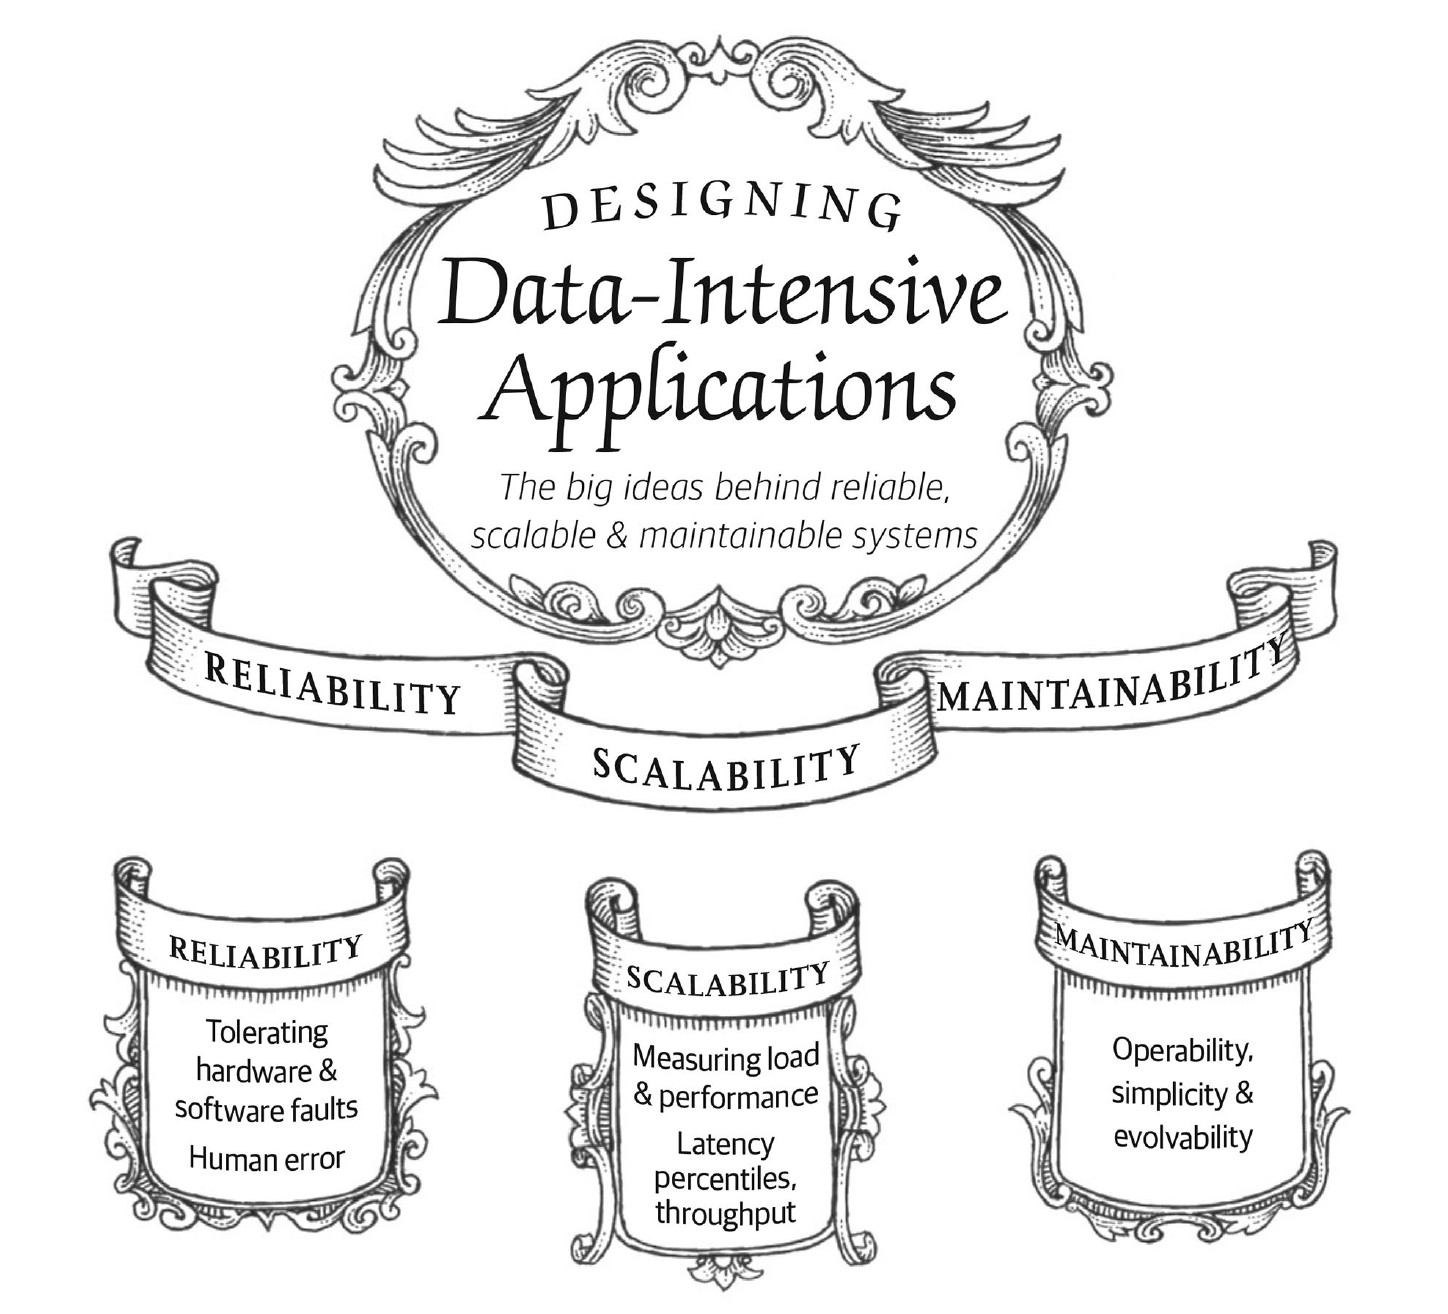
\includegraphics[scale=0.3]{dataintensiveapps.png}
\end{center}
\end{frame}
%-------------------------------------------------------------------------------------------------

%-------------------------------------------------------------------------------------------------
\begin{frame}\frametitle{Data-Intensive vs Compute-Intensive Apps}

Many applications today are \textbf{data-intensive}, as opposed to \textbf{compute-intensive}.
\\ \vfill
\emph{Raw CPU power} is rarely a limiting factor for these applications - bigger problems are
following:
\vfill
\begin{itemize}
    \item \emph{The amount of data} \vfill
    \item \emph{The complexity of data} \vfill
    \item \emph{The speed at which data is changing} \vfill
\end{itemize}
\end{frame}
%-------------------------------------------------------------------------------------------------

%-------------------------------------------------------------------------------------------------
\begin{frame}\frametitle{Data-Intensive Apps Building Blocks}
\scriptsize
A data-intensive application is typically built from \emph{standard building blocks} that provide
commonly needed functionality:
\vfill
\begin{itemize}
    \item \textbf{Databases} - Store data so that they, or another application, can find it again later. \vfill
    \item \textbf{Caches} - Remember the result of an expensive operation, to speed up reads. \vfill
    \item \textbf{Search Indexes} - Allow users to search data by keyword or filter it in various ways. \vfill
    \item \textbf{Stream Processing} - Send a message to another process, to be handled asynchronously. \vfill
    \item \textbf{Batch Processing} - Periodically crunch a large amount of accumulated data.
\end{itemize}

\end{frame}
%-------------------------------------------------------------------------------------------------

%-------------------------------------------------------------------------------------------------
\begin{frame}\frametitle{Architecture Example With Several Components}
\begin{center}
    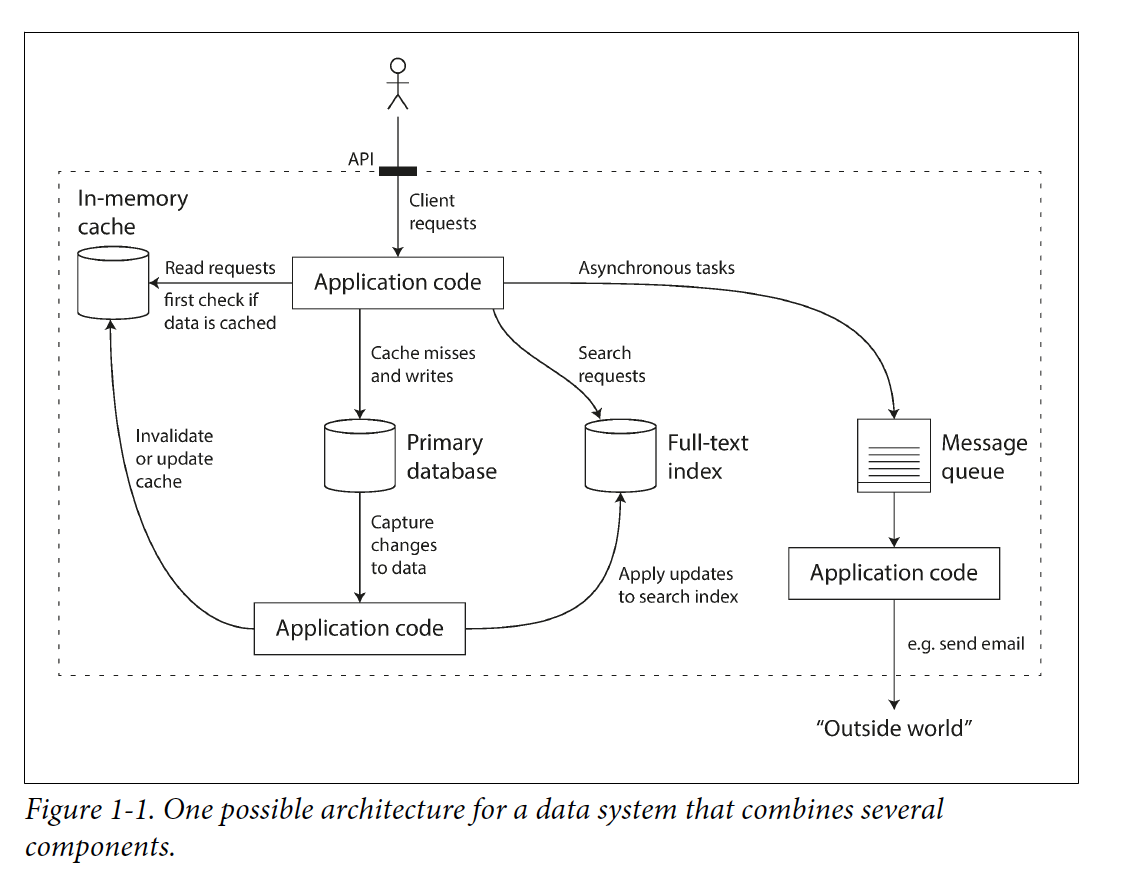
\includegraphics[scale=0.4]{exampledatasystem.png}
\end{center}
\end{frame}
%-------------------------------------------------------------------------------------------------

%-------------------------------------------------------------------------------------------------
\begin{frame}\frametitle{Thinking About Data Systems}
\scriptsize
Now you have a new, special-purpose \textbf{Data System} from smaller, general-purpose components.
\vfill
When you combine several components in order to provide a service, the service's interface
or \emph{Application Programming Interface \textbf{(API)}} usually hides implementation details from clients.
\vfill
Your composite data system may provide \textbf{certain guarantees}: \\
\emph{e.g.}, that the cache will be correctly invalidated or updated on writes so that outside
clients see consistent results.
\vfill
If you are designing a data system or service, a lot of \textbf{tricky questions} arise:
\begin{itemize}
    \item\emph{How do you ensure that the data remains correct and complete,
    even when things go wrong internally?}\\
    \item\emph{How do you provide consistently good performance to clients,
    even when parts of your system are degraded?}\\
    \item\emph{How do you scale to handle an increase in load?}\\
    \item\emph{What does a good API for the service look like?}\\
\end{itemize}
\end{frame}
%-------------------------------------------------------------------------------------------------

%-------------------------------------------------------------------------------------------------
\begin{frame}\frametitle{Reliability, Scalability and Maintainability}
\scriptsize
In this course, we focus on three concerns that are important in most software systems:
\vfill
\begin{itemize}
    \item \textbf{\textit{Reliability}} - The system should continue to work correctly
    (performing the correct function at the desired level of performance) even in the
    face of adversity (hardware or software faults, and even human error). \vfill
    \item \textbf{\textit{Scalability}} - As the system grows (in data volume, traffic volume,
    or complexity), there should be reasonable ways of dealing with that growth. \vfill
    \item \textbf{\textit{Maintainability}} - Over time, many different people will work on the
    system (engineering and operations, both maintaining current behavior and adapting the system
    to new use cases), and they should all be able to work on it productively.
\end{itemize}
\end{frame}
%-------------------------------------------------------------------------------------------------

\section{Reliability}
%-------------------------------------------------------------------------------------------------
\begin{frame}\frametitle{Reliability}
\scriptsize
For software, typical expectations for \textbf{being reliable} include:
\vfill
\begin{itemize}
    \item The application performs the function that the user expected. \vfill
    \item It can tolerate the user making mistakes or using the software
    in unexpected ways. \vfill
    \item Its performance is good enough for the required use case,
    under the expected load and data volume. \vfill
    \item The system prevents any unauthorized access and abuse. \vfill
\end{itemize}
\vfill
If all those things together mean \textbf{\textit{"working correctly"}}, then we can
understand reliability as meaning \textbf{\textit{"continuing to work correctly,
even when things go wrong"}}.
\end{frame}
%-------------------------------------------------------------------------------------------------

%-------------------------------------------------------------------------------------------------
\begin{frame}\frametitle{Faults}
\scriptsize
The things that can go wrong are called \textbf{faults}.
\vfill
Systems that anticipate faults and can cope with them are called \textbf{fault-tolerant} or \textbf{resilient}.
\vfill
The former term is slightly \emph{misleading}: it suggests that we could make
a system tolerant of every possible kind of fault, which in reality is not feasible.
\vfill
Note that a \textbf{\textit{fault}} is not the same as a \textbf{\textit{failure}}.
\vfill
A \emph{fault} is usually defined as one component of the system deviating from its spec,
whereas a \emph{failure} is when the system as a whole stops providing the required service to the user.
\vfill
It is impossible to reduce the probability of a fault to zero;
therefore it is usually best to design fault-tolerance mechanisms that prevent faults from causing failures.
\end{frame}
%-------------------------------------------------------------------------------------------------

\subsection{Hardware Faults}
%-------------------------------------------------------------------------------------------------
\begin{frame}\frametitle{Hardware Faults}
\scriptsize
\emph{Examples of hardware faults}:
\vfill
\textbf{Hard disks} crash, \textbf{RAM} becomes faulty, the \textbf{power grid} has a blackout,
someone unplugs the wrong \textbf{network cable}. These things happen all the time when you have a lot of machines.
\vfill
\emph{First response} is usually to add redundancy to the individual hardware components:
Disks may be set up in a \textbf{RAID configuration}, servers may have \textbf{dual power supplies} and
\textbf{hot-swappable CPUs}, and datacenters may have \textbf{batteries and diesel generators} for backup power.
\vfill
When one component dies, the redundant component can take its place while the broken component
is replaced. This approach cannot completely prevent hardware problems from causing failures,
but it is well understood and can often keep a machine running uninterrupted for years.
\vfill
Until recently, redundancy of hardware components was sufficient for most applications,
since it makes \emph{total failure of a single machine fairly rare}.
\end{frame}
%-------------------------------------------------------------------------------------------------

\subsection{Software Errors}
%-------------------------------------------------------------------------------------------------
\begin{frame}\frametitle{Software Errors}
\end{frame}
%-------------------------------------------------------------------------------------------------

\subsection{Human Errors}
%-------------------------------------------------------------------------------------------------
\begin{frame}\frametitle{Human Errors}
\end{frame}
%-------------------------------------------------------------------------------------------------

%-------------------------------------------------------------------------------------------------
\begin{frame}\frametitle{How Important Is Reliability?}
\end{frame}
%-------------------------------------------------------------------------------------------------

\section{Scalability}
%-------------------------------------------------------------------------------------------------
\begin{frame}\frametitle{Scalability}
\end{frame}
%-------------------------------------------------------------------------------------------------

\subsection{Describing Load}
%-------------------------------------------------------------------------------------------------
\begin{frame}\frametitle{Describing Load}
\end{frame}
%-------------------------------------------------------------------------------------------------

\subsection{Describing Performance}
%-------------------------------------------------------------------------------------------------
\begin{frame}\frametitle{Describing Performance}
\end{frame}
%-------------------------------------------------------------------------------------------------

\subsection{Approaches for Coping with Load}
%-------------------------------------------------------------------------------------------------
\begin{frame}\frametitle{Approaches for Coping with Load}
\end{frame}
%-------------------------------------------------------------------------------------------------

\section{Maintainability}
%-------------------------------------------------------------------------------------------------
\begin{frame}\frametitle{Maintainability}
\end{frame}
%-------------------------------------------------------------------------------------------------

\subsection{Operability: Making Life Easy for Operations}
%-------------------------------------------------------------------------------------------------
\begin{frame}\frametitle{Operability: Making Life Easy for Operations}
\end{frame}
%-------------------------------------------------------------------------------------------------

\subsection{Simplicity: Managing Complexity}
%-------------------------------------------------------------------------------------------------
\begin{frame}\frametitle{Simplicity: Managing Complexity}
\end{frame}
%-------------------------------------------------------------------------------------------------

\subsection{Evolvability: Making Change Easy}
%-------------------------------------------------------------------------------------------------
\begin{frame}\frametitle{Evolvability: Making Change Easy}
\end{frame}
%-------------------------------------------------------------------------------------------------

%-------------------------------------------------------------------------------------------------
\begin{frame}\frametitle{Summary}
\end{frame}
%-------------------------------------------------------------------------------------------------

\end{document}
